Um exemplo de equação característica é a equação (\ref{eq:termistor}), do termistor, que será utilizada nesta seção. Os dados gerados para o gráfico \ref{fig:escala:semilog:dados} continuarão os mesmos aqui.

\subsection{Encontrando os Coeficientes}

    O primeiro passo normalmente é encontrar os coeficientes da equação característica. Se for uma equação de reta, uma simples regressão linear é bastante para encontrar esses coeficientes e para mostrar a equação esperada. Para os outros caso, no entanto, é preciso linearizar a equação, como foi feito na seção \nameref{sec:escala}, encontrar os coeficientes da linearização e transformar para os coeficientes da equação inicial.

    No caso dos dados do termistor, a regressão é aplicada como na figura \ref{fig:caract:regres}. Logo, os coeficientes se tornam $A = \exp(-7.07097) \approxeq 0.00084941$ e $B = 4632.762$.

    \begin{figure}[htbp]
        \centering
        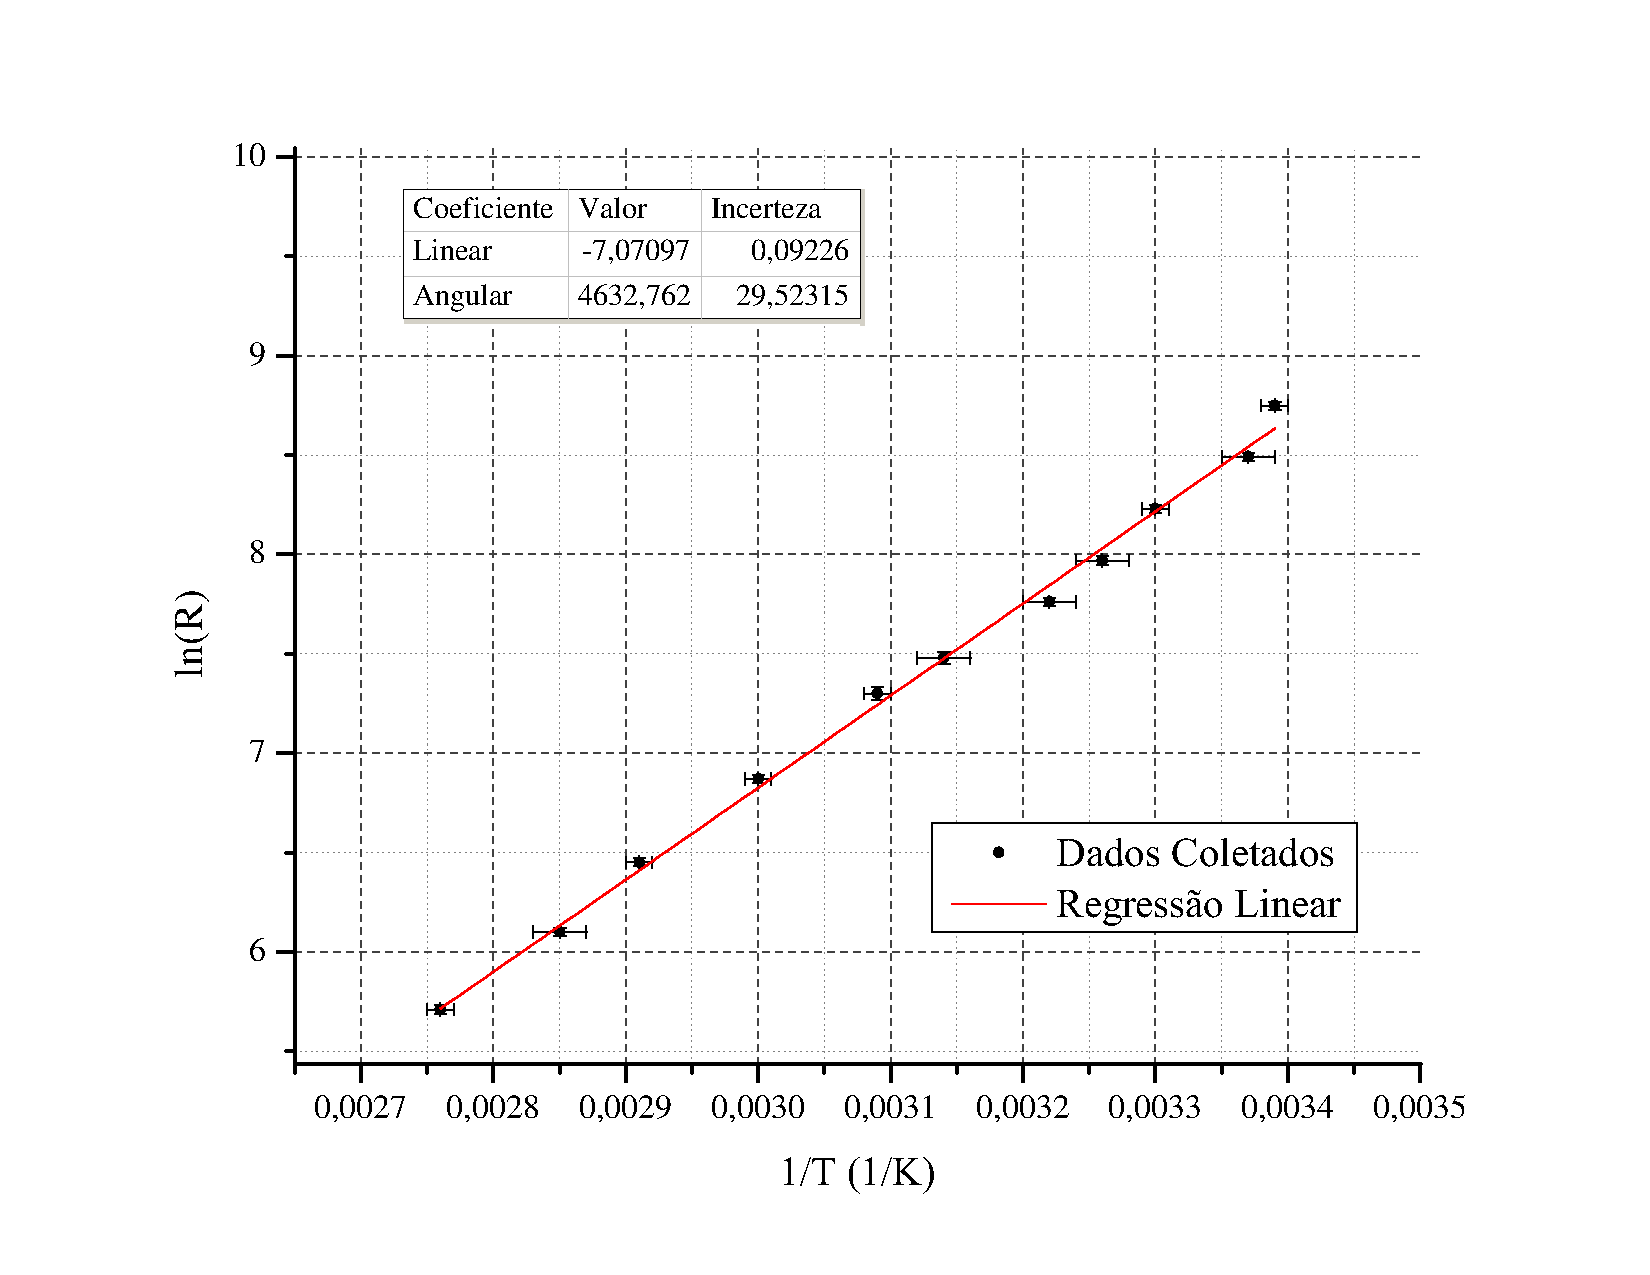
\includegraphics[width=0.8\textwidth]{caract/1regres.pdf}

        \caption{Gráfico da linearização da equação (\ref{eq:termistor})}
        \label{fig:caract:regres}
    \end{figure}


    \subsection{Gráfico de Funções}

    Voltando para os dados originais, de $R$ por $T$, podemos desenhar a equação característica, agora com os valores dos coeficientes, sobre o \texttt{Scatter} dos dados, como mostra a figura \ref{fig:caract:inserir}.

    \begin{figure}[htbp]
        \centering
        \begin{subfigure}{0.32\textwidth}
            \centering
            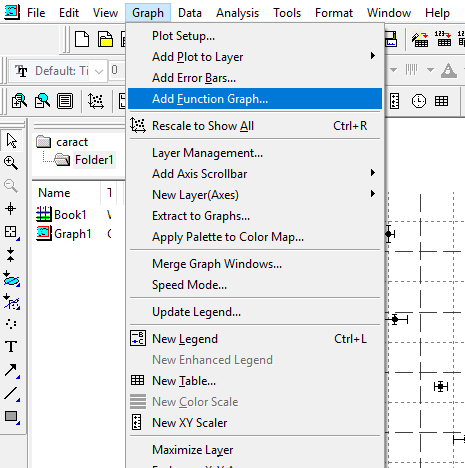
\includegraphics[width=\textwidth]{caract/2insert.png}

            \caption{Adicionando uma função no gráfico}
            \label{fig:caract:novo}
        \end{subfigure}
        ~
        \begin{subfigure}{0.63\textwidth}
            \centering
            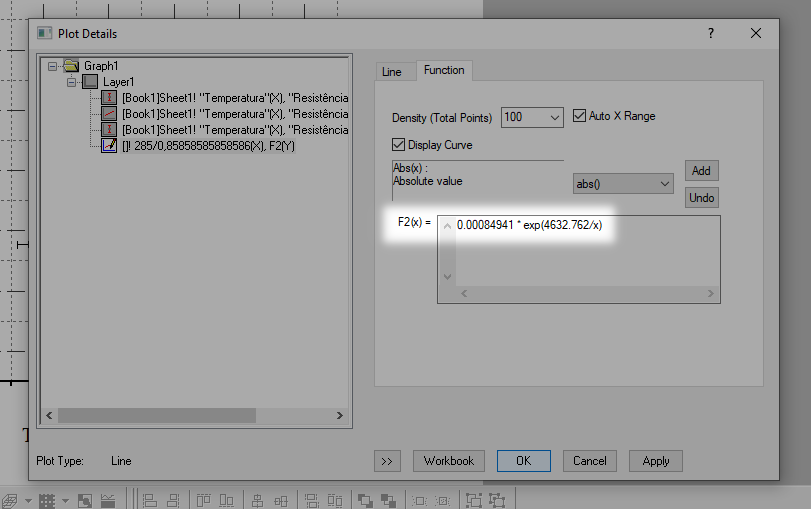
\includegraphics[width=\textwidth]{caract/4funcao.png}

            \caption{Colocando a função $R = 0.00084941 ~ \exp(4632.762/T)$}
            \label{fig:caract:funcao}
        \end{subfigure}
        \caption{Desenhando uma função no gráfico}
        \label{fig:caract:inserir}
    \end{figure}


\subsection{Ajustes de Formatação}

    Por padrão, a cor da nova curva do gráfico é escolhida como preto, mas isso pode ser mudado com um duplo clique sobre a curva. Neste exemplo a cor decidida foi vermelho, que acompanha o padrão de regressão dos exemplos anteriores.

    \begin{figure}[htbp]
        \centering
        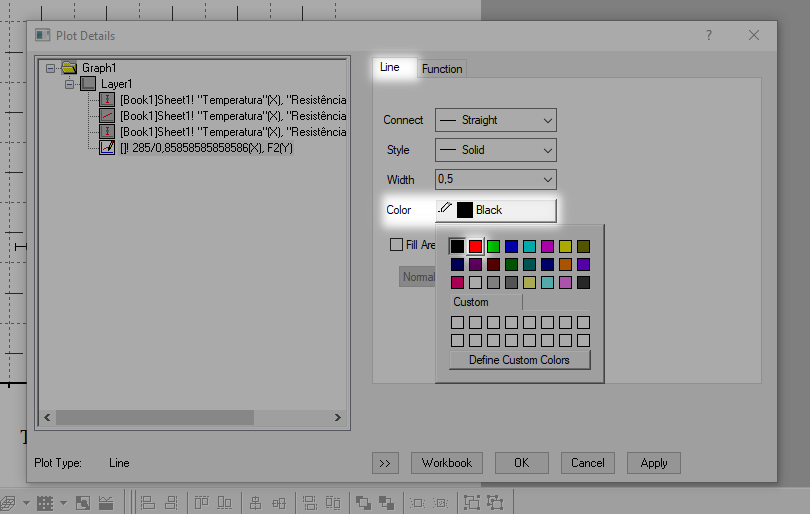
\includegraphics[width=0.8\textwidth]{caract/5cor.png}

        \caption{Mudança da cor da nova curva}
        \label{fig:caract:cor}
    \end{figure}

    Além da cor, é importante lembrar de tratar da curva na legenda do gráfico, caso isso não tenha sido feito automaticamente, que pode ser feito pelas propriedades da legenda. Normalmente, a descrição da curva pode ser dada também pela sua forma algébrica.

    \begin{figure}[htbp]
        \centering
        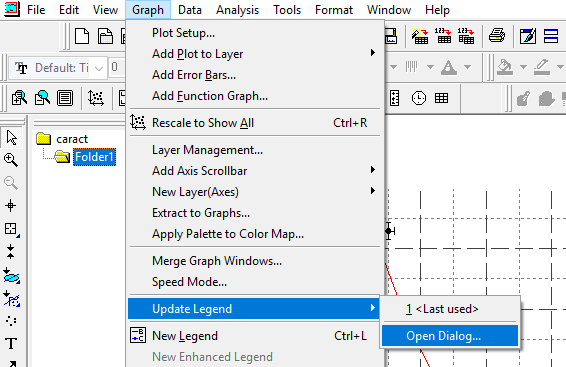
\includegraphics[width=0.7\textwidth]{caract/6leg.png}
        \caption{Atualizando a legenda com a nova curva}
        \label{fig:caract:legenda}
    \end{figure}


\subsection{Resultado}

    \begin{figure}[htbp]
        \centering
        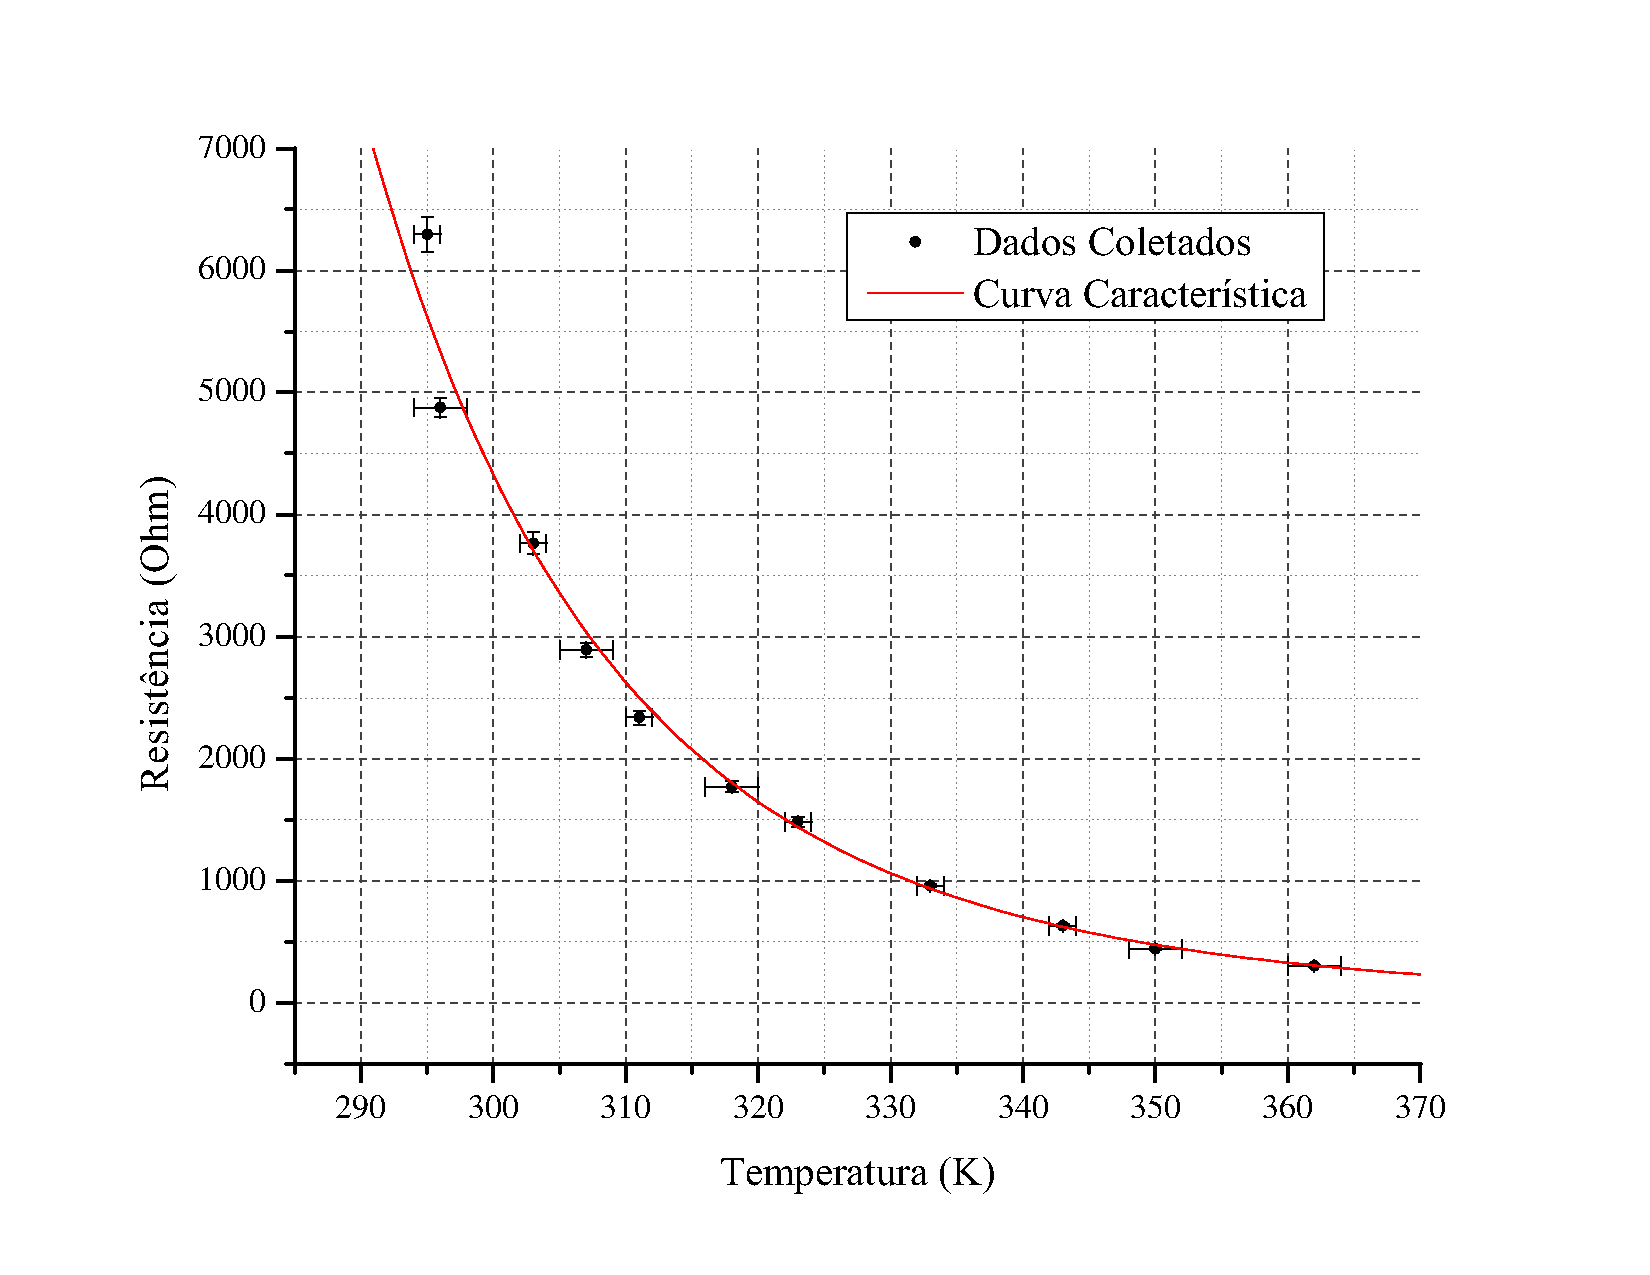
\includegraphics[width=0.8\textwidth]{caract/8final.pdf}

        \caption{Gráfico com a curva característica do termistor}
        \label{fig:caract:final}
    \end{figure}
